Процесс состоит из нескольких частей:
\begin{enumerate}
    \item Сбор опций пользователя при помощи интерактивного диалога
    \item Поиск опций в хранилище
    \item По путям из хранилища программа осуществляет поход в интернет и
          загрузку кодов алгоритмов
    \item Загруженные алгоритмы записываются на ФС машины
    \item Загруженные алгоритмы устанавливаются в систему
    \item На ФС записываются функции, обеспечивающие совместимость выбранных
          пользователем алгоритмов и реализации блокчейна
    \item На ФС записывается реализация блокчейна
\end{enumerate}

Процессы будут описываться по порядку, начиная со сбора опций.

\subsubsection{Сбор опций пользователя}

Начинается с отображения приветственного и инструкционного сообщения (Рис. \ref{dg_st})

\begin{figure}[h]
    \centering
    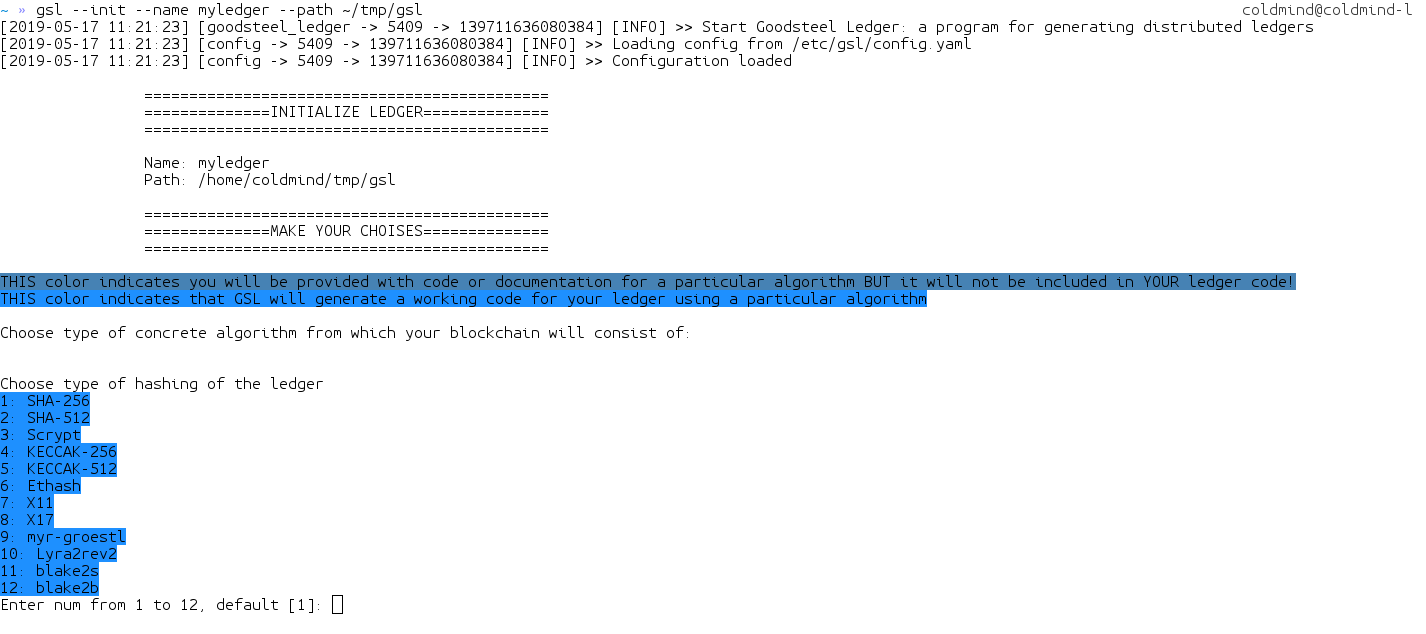
\includegraphics[width=\textwidth]{images/dialog_start}
    \caption{Начало работы компоновщика: приветственное окно и первый набор алгоритмов}\label{dg_st}
\end{figure}

В листинге \ref{print_opts} описан процесс сбора опций пользователя. Из
хранилища берётся список всех возможных опций, и согласно порядку типов
алгоритмов, распечатываются в пронумерованном виде соответствующие опции.
Пользователь затем вводит номер, размах значений которого соответствует опциям
алгоритмов данного типа. Предусмотрено значение ``по умолчанию'' для каждой из
опций --- первое значение. Вывод алгоритмов раскрашивается --- из
реализованного в рамках данной работы \textbf{utils} были импортированы функции
и константы для форматирования вывода. В случае ошибки в стандартный выход
логгера выводится её сообщение.
\begin{center}
\begin{lstlisting}
    for k, v in OPTIONS.items():
        print(f'\nChoose type of {k} of the ledger')
        if isinstance(v, list):
            for num, opt in enumerate(v):
                if 'hash' in k or 'digital' in k:
                    if opt in TOINSTALL:
                        prefix = ASCIIColors.BACK_BLUE
                    else:
                        prefix = ASCIIColors.BACK_LIGHT_BLUE
                else:
                    prefix = ASCIIColors.ENDS
                print(f'{prefix}{num+1}: {opt}{ASCIIColors.ENDS}', end='\n')
            try:
                n = input(f'Enter num from 1 to {len(v)}, default [1]: ')
                n = 0 if n == '' else int(n) - 1
                if n < 0 or n >= len(v):
                    raise ChooseError
                self.ledger_config[k] = n
            except Exception as e:
                __logger__.exception(str(e))
                return
        else:
            print(v)
\end{lstlisting}\label{print_opts}
    Листинг \ref{print_opts}: Процесс выбора опций пользователем
\end{center}

\subsubsection{Поиск алгоритмов}
На данный момент выбранные пользователем опции были получены, и записаны в переменную \textbf{options}.
Поиском алгоритмов в хранилище, интернете и их установкой на ФС машины занимается класс \textbf{ProlificWriter}.

Процесс поиска ссылок для алгоритмов в хранилище происходит путём поиска
соответствий переданных классу опций с полем хранилища \emph{TOINSTALL}. Запись
на ФС установленных алгоритмов происходит в методе \textbf{write}. Сначала
пишутся алгоритмы хэширования и электронной подписи, а затем --- код реализации
блокчейна.

\begin{center}
\begin{lstlisting}
    def write(self):
        # WRITE ALGORITHMS ITSELF
        #
        self._write_hashing_()
        self._write_digital_signature_()

        self._write_(wallet)
        self._write_(miner)


    def _write_(self, script_to_write):
        name = f'{script_to_write.__name__.split(".")[-1]}.py'
        src_code = getsource(script_to_write)
        with open(os.path.join(self.path, name), 'w') as __fd__:
            __fd__.write(src_code)
        if self.timed:
            os.system('sed -ir "0,/def _timed/{s/_timed = .*/_timed = True/}" ' + os.path.join(self.path, name))
        if self.profd:
            os.system('sed -ir "0,/def _profd/{s/_profd = .*/_profd = True/}" ' + os.path.join(self.path, name))


    def _write_hashing_(self):
        # INSTALLING PROCEDURE
        src_path = self._get_src_path_()
        path = os.path.join(src_path, get('TOINSTALL', self.opts['hashing']))
        self._install_(path)

        # WRITING PROCEDURE
        name = 'myhashing.py'
        type_ = self.opts['hashing']
        path = os.path.join(src_path, get('INTERFACES', type_), name)
        if not os.path.exists(self.path):
            os.makedirs(self.path)
        copyfile(path, os.path.join(self.path, name))

    def _write_digital_signature_(self):
        # INSTALLING PROCEDURE
        src_path = self._get_src_path_()
        path = os.path.join(src_path, get('TOINSTALL', self.opts['digital signature']))
        self._install_(path)

        # WRITING PROCEDURE
        name = 'mydss.py'
        type_ = self.opts['digital signature']
        path = os.path.join(src_path, get('INTERFACES', type_), name)
        copyfile(path, os.path.join(self.path, name))
\end{lstlisting}\label{write}
    Листинг \ref{write}: Процесс поиска алгоритмов и записи на ФС машины
\end{center}

\subsubsection{Установка}
Установка алгоритмов, упомянутая до этого в листинге \ref{write}, происходит
посредством запуска метода \_install\_, а при неудачной попытки ---
\_pip\_install\_.

\begin{center}
\begin{lstlisting}
    def _install_(self, path):
        """
        Installs with `python setup.py install`
        """
        os.chdir(path)
        subprocess.call([sys.executable, f'{path}/setup.py', 'install'])


    def _pip_install_(self, package):
        subprocess.call([sys.executable, '-m', 'pip', 'install', package, '--user'])
\end{lstlisting}\label{lst:inst}
Листинг \ref{lst:inst}: Код для установки алгоритмов на ФС машины
\end{center}


\subsubsection{Запись реализации блокчейна}

Запись на ФС методов-обёрток для совместимости выбранных пользователем
алгоритмов и реализации блокчейна, содержится в листинге \ref{write}. За запись
методов-обёрток отвечает метод \textbf{\_write\_hashing\_} и
\textbf{\_write\_digital\_signature\_}.


